\documentclass[a4paper,5pt]{amsbook}
%%%%%%%%%%%%%%%%%%%%%%%%%%%%%%%%%%%%%%%%%%%%%%%%%%%%%%%%%%%%%%%%%%%%%

\usepackage{booktabs}
\usepackage{graphicx}
\usepackage{multicol}
\usepackage{textcomp}
\usepackage{systeme}
\usepackage{amssymb}
\usepackage[]{amsmath}
\usepackage{subcaption}
\usepackage[inline]{enumitem}
\usepackage{gensymb}

%%%%%%%%%%%%%%%%%%%%%%%%%%%%%%%%%%%%%%%%%%%%%%%%%%%%%%%%%%%%%%

\newcommand{\sen}{\,\mbox{sen}}
\newcommand{\tg}{\,\mbox{tg}\,}
\newcommand{\cosec}{\,\mbox{cosec}\,}
\newcommand{\cotg}{\,\mbox{cotg}\,}
\newcommand{\tr}{\,\mbox{tr}\,}
\newcommand{\ds}{\displaystyle}

%%%%%%%%%%%%%%%%%%%%%%%%%%%%%%%%%%%%%%%%%%%%%%%%%%%%%%%%%%%%%%%%%%%%%%%%

\setlength{\textwidth}{16cm} %\setlength{\topmargin}{-1.3cm}
\setlength{\textheight}{21cm}
\setlength{\leftmargin}{1.2cm} \setlength{\rightmargin}{1.2cm}
\setlength{\oddsidemargin}{0cm}\setlength{\evensidemargin}{0cm}

%%%%%%%%%%%%%%%%%%%%%%%%%%%%%%%%%%%%%%%%%%%%%%%%%%%%%%%%%%%%%%%%%%%%%%%%

% \renewcommand{\baselinestretch}{1.6}
% \renewcommand{\thefootnote}{\fnsymbol{footnote}}
% \renewcommand{\theequation}{\thesection.\arabic{equation}}
% \setlength{\voffset}{-50pt}
% \numberwithin{equation}{chapter}

%%%%%%%%%%%%%%%%%%%%%%%%%%%%%%%%%%%%%%%%%%%%%%%%%%%%%%%%%%%%%%%%%%%%%%%

\begin{document}
\thispagestyle{empty}
\pagestyle{empty}
\begin{minipage}[h]{0.14\textwidth}
	
\includegraphics[scale=0.24]{../ufgd.png}
\end{minipage}
\begin{minipage}[h]{\textwidth}
\begin{tabular}{c}
{{\bf UNIVERSIDADE FEDERAL DA GRANDE DOURADOS}}\\
{{\bf C\'alculo Diferencial e Integral --- Lista 3}}\\
{{\bf Prof.\ Adriano Barbosa}}\\
\end{tabular}
\vspace{-0.45cm}
%
\end{minipage}

%------------------------

\vspace{1cm}
%%%%%%%%%%%%%%%%%%%%%%%%%%%%%%%%   formulario  inicio  %%%%%%%%%%%%%%%%%%%%%%%%%%%%%%%%
\begin{enumerate}
    \vspace{0.5cm}
    \item Para $f$ e $g$ abaixo, verifique se $f=g$.
        \begin{enumerate}
            \vspace{0.3cm}
            \item $f(x)=x+\sqrt{2-x}$ e $g(u)=u+\sqrt{2-u}$.
            \vspace{0.3cm}
            \item $f(x)=\displaystyle \frac{x^2-x}{x-1}$ e $g(x)=x$.
        \end{enumerate}

    \vspace{0.5cm}
    \item Determine se as curvas abaixo s\~ao gr\'afico de uma fun\c{c}\~ao de $x$
        \begin{figure}[h]
            \centering
            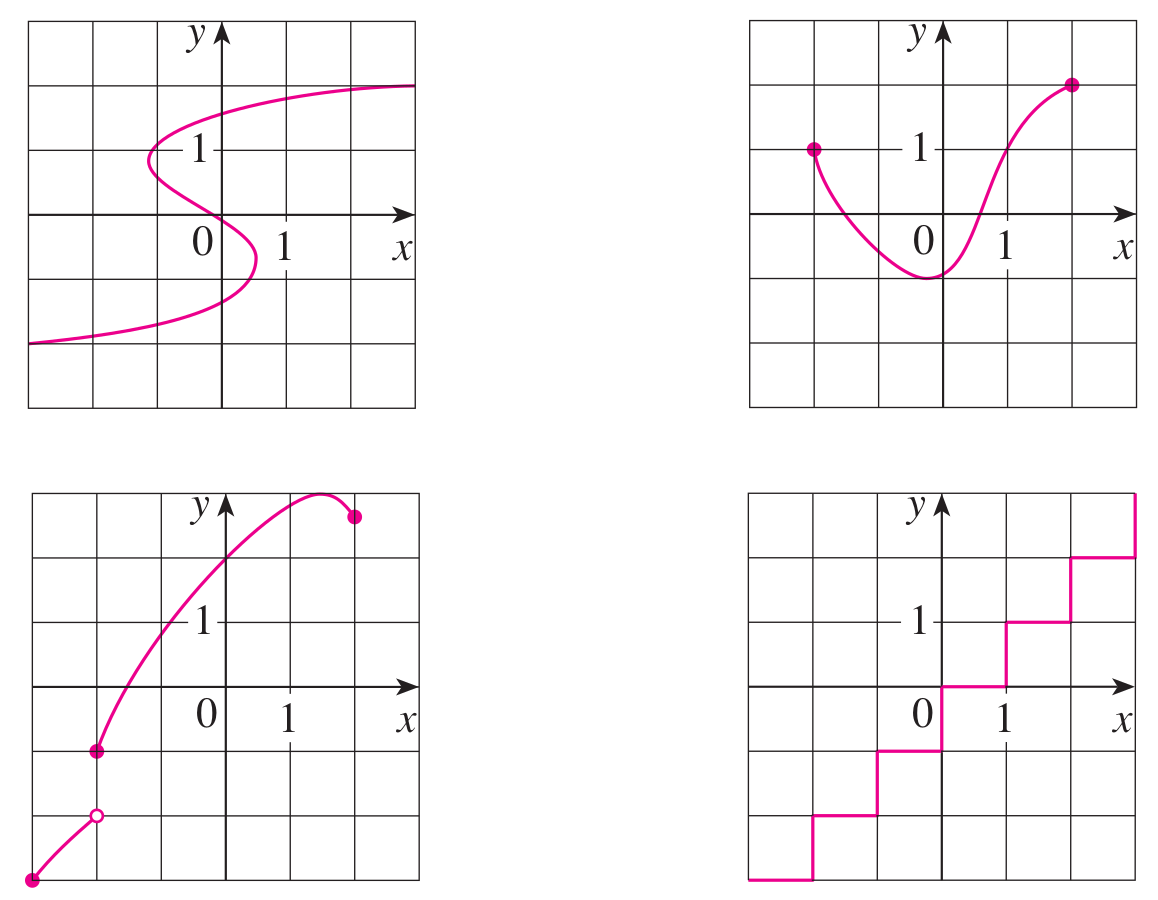
\includegraphics[width=0.5\textwidth]{lista-03-fig1.png}
        \end{figure}

    \vspace{0.5cm}
    \item Determine o maior dom\'{\i}nio das fun\c{c}\~oes abaixo:
        \begin{enumerate}
            \vspace{0.3cm}
            \item $\displaystyle f(x)=\frac{x+4}{x^2-9}$
            \vspace{0.3cm}
            \item $f(t)=\sqrt[3]{2t-1}$
            \vspace{0.3cm}
            \item $f(x)=\displaystyle\frac{2x^3-5}{x^2+x-6}$
            \vspace{0.3cm}
            \item $f(t)=\sqrt{3-t}-\sqrt{2+t}$
        \end{enumerate}

    \vspace{0.5cm}
    \item De um peda\c{c}o retangular de cartolina de dimens\~oes $8$cm$\times 15$cm,
        quatro quadrados iguais devem ser cortados, um em cada canto. A parte
        cortada remanescente \'e ent\~ao dobrada formando uma caixa aberta.
        Expresse o volume da caixa como uma fun\c{c}\~ao de $x$.

    \vspace{0.5cm}
    \item A rela\c{c}\~ao entre as escalas de temperatura Celsius (C) e Fahrenheit
        (F) \'e dada pela fun\c{c}\~ao afim $F=\displaystyle\frac{9}{5}C+32$. Desenhe o
        gr\'afico dessa fun\c{c}\~ao. Encontre o intervalo na escala F correspondente
        as temperaturas em C que est\~ao entre $18\degree$ C e $25\degree$ C.

    \vspace{0.5cm}
    \item Encontre a express\~ao para as fun\c{c}\~oes quadr\'aticas cujos gr\'aficos s\~ao:
        \begin{figure}[h]
            \centering
            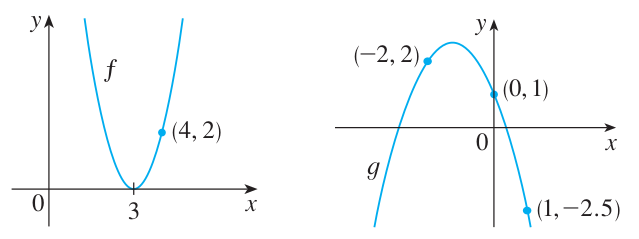
\includegraphics[width=0.5\textwidth]{lista-03-fig2.png}
        \end{figure}

    \vspace{0.5cm}
    \item Desenhe o gr\'afico das fun\c{c}\~oes abaixo a partir de um gr\'afico conhecido
        e aplicando transla\c{c}\~oes e escalas nos eixos $x$ e $y$.
        \begin{enumerate}
            \vspace{0.3cm}
            \item $y=\displaystyle\frac{1}{x+2}$
            \vspace{0.3cm}
            \item $y={(x-1)}^3$
            \vspace{0.3cm}
            \item $y=x^2+6x+4$
            \vspace{0.3cm}
            \item $y=|x|-2$
            \vspace{0.3cm}
            \item $y=\sen\left(\displaystyle\frac{1}{2}x\right)$
            \vspace{0.3cm}
            \item $y=\displaystyle\frac{1}{2}\left(1-\cos(x)\right)$
        \end{enumerate}

    \vspace{0.5cm}
    \item Encontre as regras das fun\c{c}\~oes $f\circ g$ e $g\circ f$ e determine
        seus dom\'{\i}nios.
        \begin{enumerate}
            \vspace{0.3cm}
            \item $f(x)=x^2-1$ e $g(x)=2x+1$
            \vspace{0.3cm}
            \item $f(x)=x-2$ e $g(x)=x^2+3x+4$
            \vspace{0.3cm}
            \item $f(x)=x+\displaystyle\frac{1}{x}$ e $g(x)=\displaystyle\frac{x+1}{x+2}$
            \vspace{0.3cm}
            \item $f(x)=\displaystyle\frac{x}{1+x}$ e $g(x)=\sen(2x)$
        \end{enumerate}
\end{enumerate}

\end{document}
